\documentclass{beamer}
\usetheme{default}

\usepackage{subfigure}
\usepackage{amsmath}
\usepackage{gensymb}

\begin{document}

\begin{frame}{}

\title{\textbf{Image Processing}}
\maketitle

Chloe Eghtebas, Luke Metz, Brendan Ritter

\end{frame}


\begin{frame}{Basics of Image Processing}

Using computational software to manipulate an image using signal processing techniques. 

It's applications: 
Biomedical Imaging
 Recognition and Tracking

\end{frame}



\begin{frame}{What You'll Need to Know}

\begin{itemize}
		
	\item[1]Image Compression
	\item SVD
	\item[2]"Signal Processing" 
	\item Shear
    \item brightness and contrast 
    \item grayscale
    \item invert
    \item Rotating
    	\item Flipping
    \item[3]Edge Detection 
    \item Gaussian blur
    \item Sobel/convolution
\end{itemize}
\end{frame}

\begin{frame}{Image Representation and Software}

\begin{figure}
\begin{center}
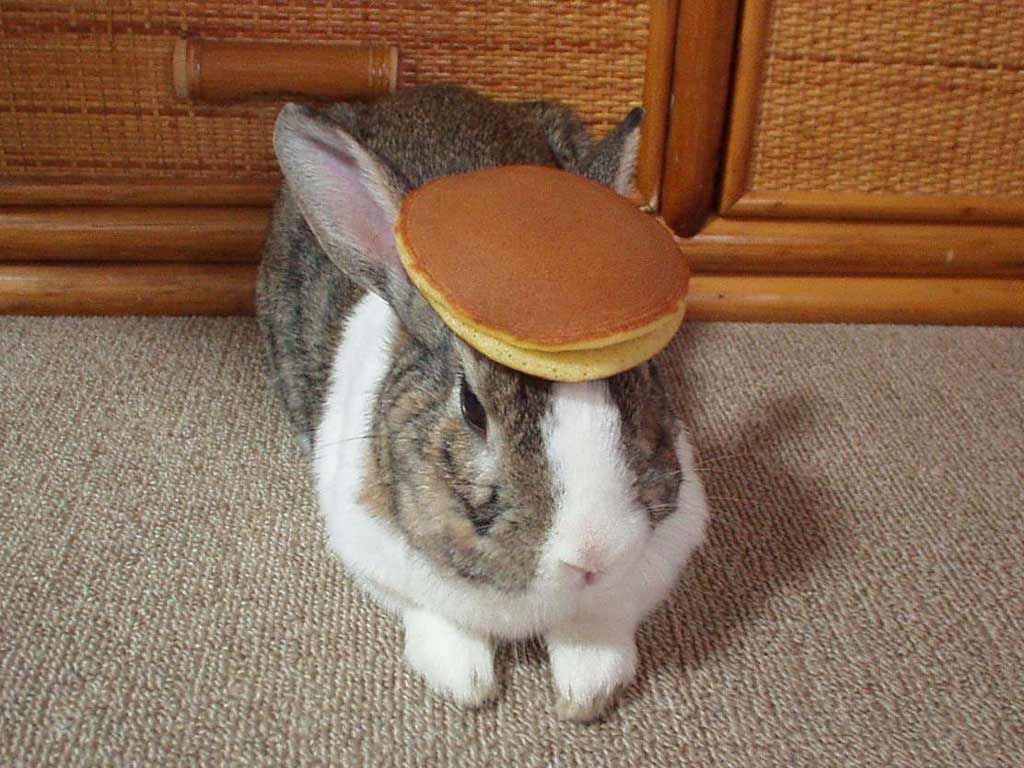
\includegraphics[width = 0.75 in]{bunny.jpg}
\end{center}
\end{figure}

Images have 3 channels. Red, Blue, Green. To manipulate these arrays we chose to not use matlab. We chose to use Python and Numpy mainly for its re usability.

\begin{figure}
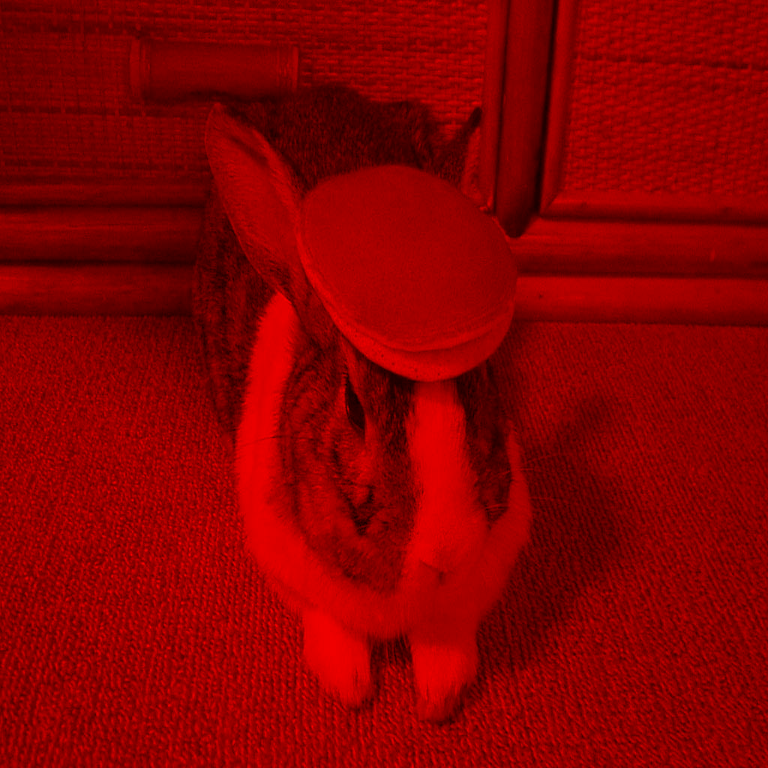
\includegraphics[width = 0.75 in]{bunnyred.png}
\hspace{0.5 in}
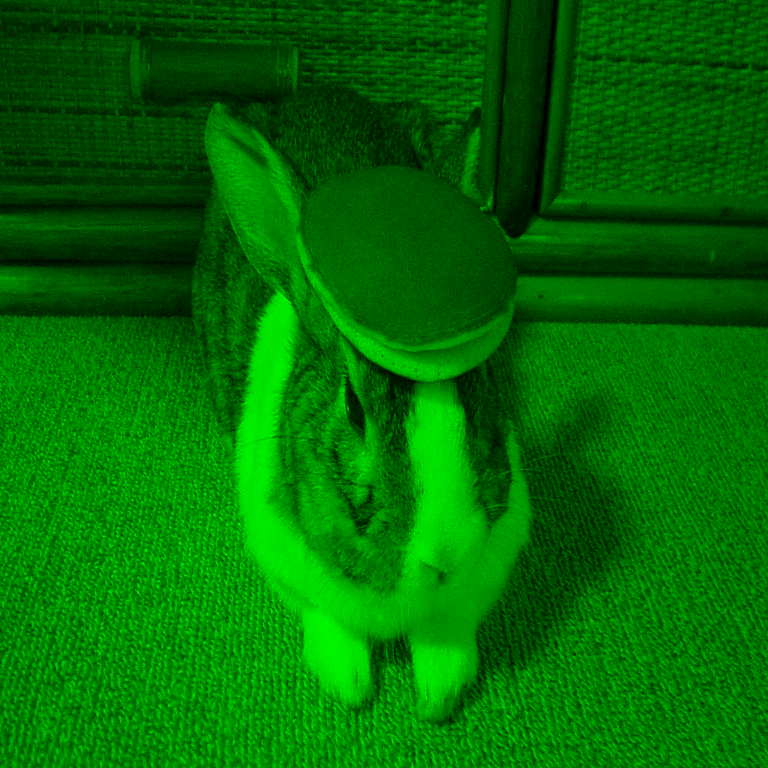
\includegraphics[width = 0.75 in]{bunnygreen.png}
\hspace{0.5 in}
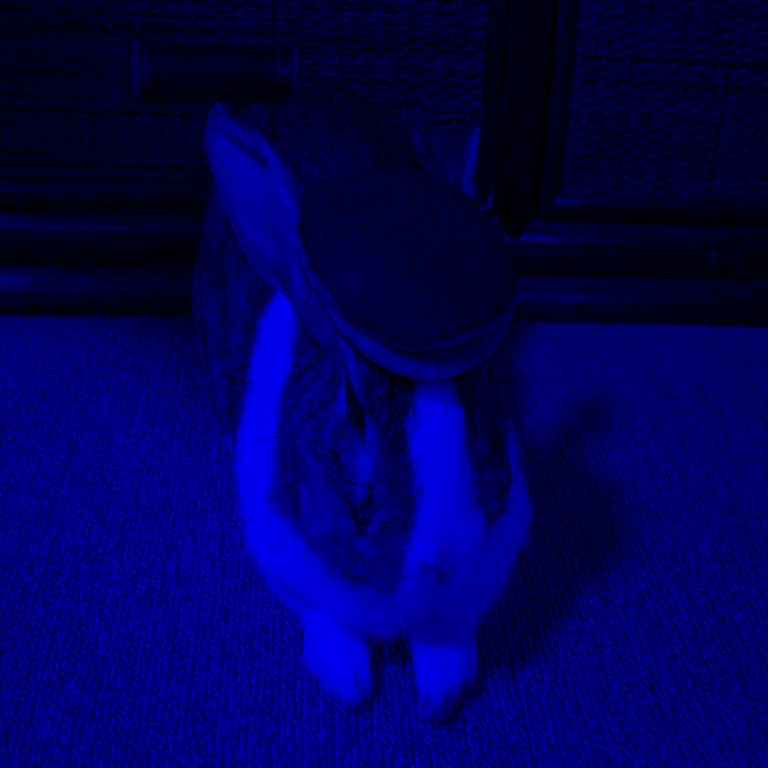
\includegraphics[width = 0.75 in]{bunnyblue.png}
\end{figure}

\end{frame} 


\begin{frame}{Flipping}


\begin{figure}
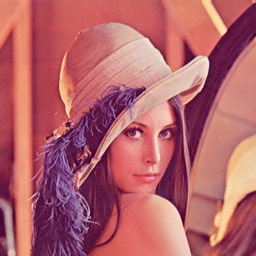
\includegraphics[width = 1.25 in]{lennastory.jpg}

\hspace{0.5 in}
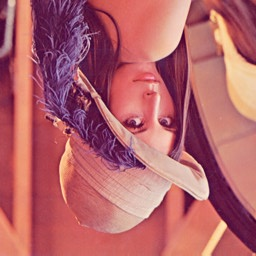
\includegraphics[width = 1.25 in]{lenna1.png}
\hspace{0.5 in}
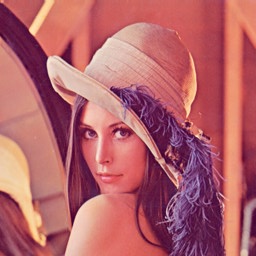
\includegraphics[width = 1.25 in]{lenna2.png}
\hspace{0.5 in}
\end{figure}

\end{frame}


\begin{frame}{Transformations}
To apply more complicated transformations to the image one first has to re arrange the image. Currently x and y position are stored at the index of the matrix. This gives us no easy way to manipulate them.

We can rearrange The image to look like:
$$A = \begin{pmatrix}
	x & 0 & ...\\
	y & 0 & ...\\
	1 & 1 & ...\\
	r &  255 & ...\\
	g & 255 & ...\\
	b & 255 & ...\\
\end{pmatrix}$$
This will let us translate, rotate, scale, and shear the image in any way.

\end{frame}

\begin{frame}{Rotation}
Example Rotation:
The Default rotation is always around the origin. To make that the center of the image, one must first translate, rotate, then translate back.
\hspace{0.1 in}
\\
$A_{out} = \begin{pmatrix}
	1 & 0 & dx\\
	0 & 1 & dy\\
	0 & 0 & 1\\
\end{pmatrix}$
$\begin{pmatrix}
	\cos(\theta) & -\sin(\theta) & 0\\
	\sin(\theta)& \cos(\theta) & 0\\
	0 & 0 & 1\\
\end{pmatrix}$
$\begin{pmatrix}
	1 & 0 & -dx\\
	0 & 1 & -dy\\
	0 & 0 & 1\\
\end{pmatrix}$
$A$
\\
\begin{figure}


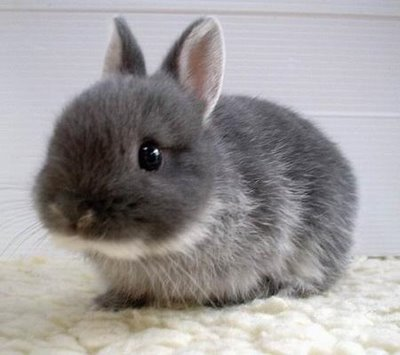
\includegraphics[width = 1.1 in]{bunnycute.jpg}
\hspace{0.5 in}
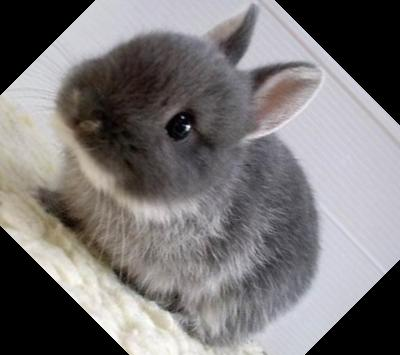
\includegraphics[width = 1.1 in]{bunnycuteRot.jpg}
\caption{Rotated around the center at $\theta = 45\degree$}
\end{figure}
\end{frame}


\begin{frame}{Rotation}
Example Rotation:
The Default rotation is always around the origin. To make that the center of the image, one must first translate, rotate, then translate back.
\hspace{0.1 in}
\\
$A_{out} = \begin{pmatrix}
	1 & \lambda_y & 0\\
	\lambda_x & 1 & 0\\
	0 & 0 & 1\\
\end{pmatrix}$
$A$
\\
\begin{figure}

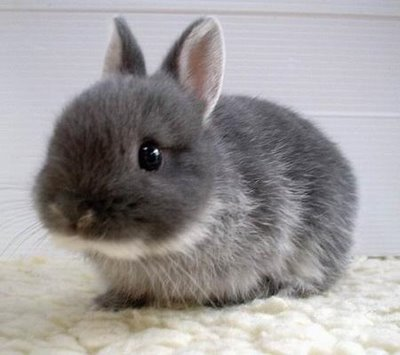
\includegraphics[width = 1.1 in]{bunnycute.jpg}
\hspace{0.5 in}
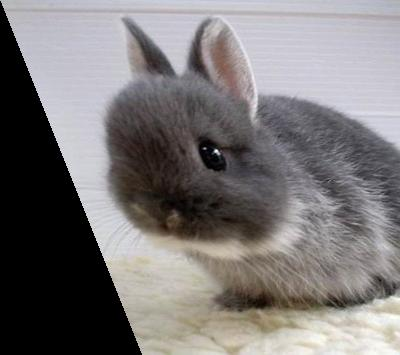
\includegraphics[width = 1.1 in]{bunnycuteShear.jpg}
\caption{Sheared with $\lambda_X = .4$ and $\lambda_Y = 0$}
\end{figure}

\end{frame}




\begin{frame}{Convolution}
'Blending' two functions together. For discrete data, its like overlapping.
One has original data and a kernel which represents the other function. 
\begin{figure}[htp]
\centering
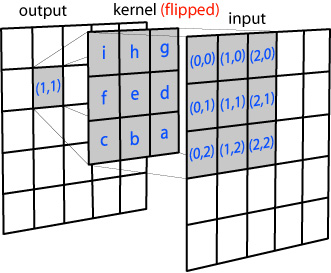
\includegraphics[width=2in]{conv2d_matrix.jpg}
\caption{Convolution in 2D.}
\label{}
\end{figure}
\end{frame}

\begin{frame}{Gaussian Blur}

Gaussian blur is an application of  convolution. It 'blends' a Gaussian, a normal curve onto the image. One has control over blurriness by the standard deviation, $\sigma$.

%\begin{figure}[ht]
%\begin{minipage}[b]{0.1\linewidth}
%\centering
%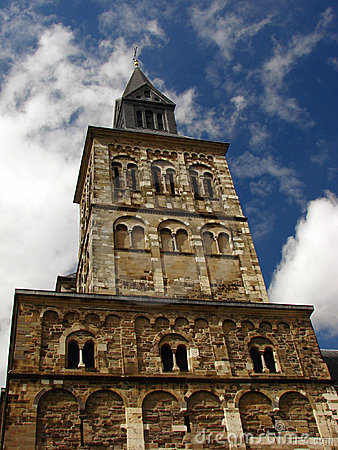
\includegraphics[width=1.3in]{churchin.jpg}
%\caption{Default Image}
%\label{fig:figure1}
%\end{minipage}
%\hspace{2.0in}
%\begin{minipage}[b]{0.1\linewidth}
%\centering
%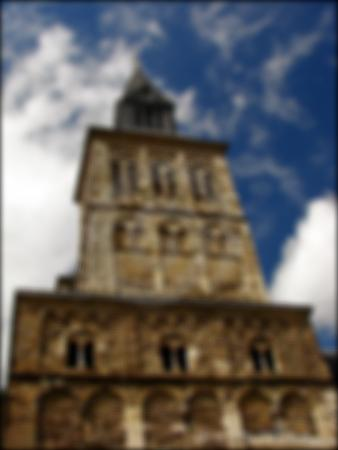
\includegraphics[width=1.3in]{churchoutb.jpg}
%\caption{Blurred Image}
%\hspace{1.0in}
%\label{fig:figure2}
%\end{minipage}
%\end{figure}

\begin{figure}[ht]
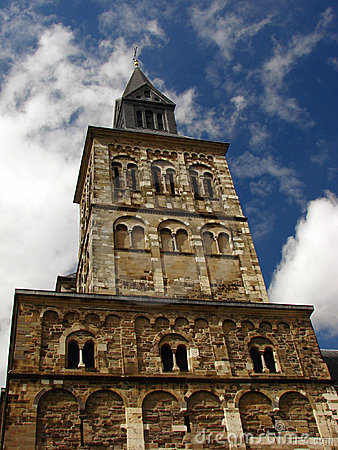
\includegraphics[width=1.3in]{churchin.jpg}
\hspace{.1in}
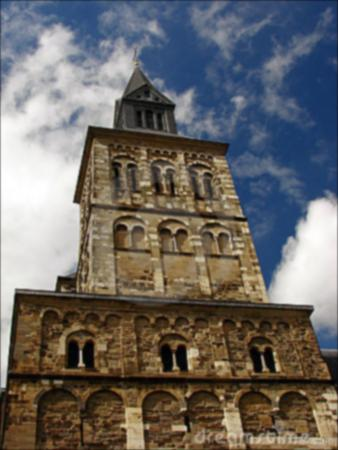
\includegraphics[width=1.3in]{churchoutblur.jpg}
\hspace{.1in}
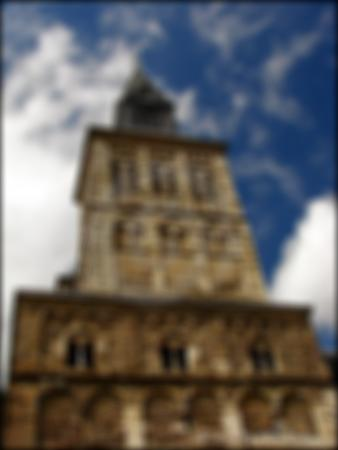
\includegraphics[width=1.3in]{churchoutblur2.jpg}
\caption{Original image on left. $\sigma$ = 2 in middle. $\sigma$ = 4 on left.}
\end{figure}


\end{frame}

\begin{frame}{Sobel Edge Detection}
Another application of convolution is edge detection. The Sobel operator can be thought of as a discrete differentiation operator. It gets how fast one color goes to another. 

\begin{figure}[ht]

\includegraphics[width=1.4in]{edgein.png}
\hspace{.1in}
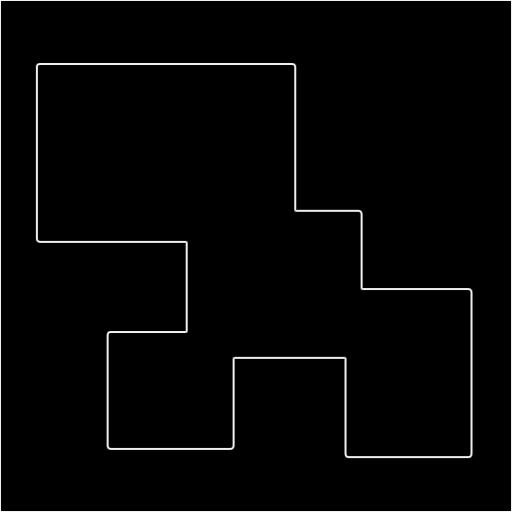
\includegraphics[width=1.4in]{edgeout.jpg}
\hspace{.1in}
\end{figure}
\end{frame}

\begin{frame}{Example}
\begin{figure}[ht]
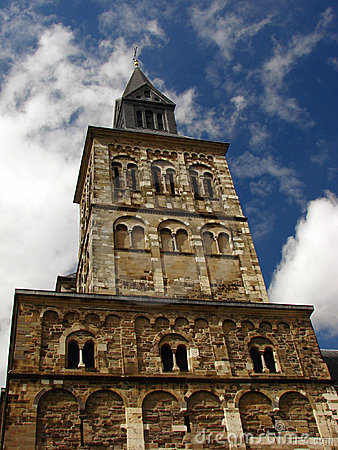
\includegraphics[width=1.4in]{churchin.jpg}
\hspace{.1in}
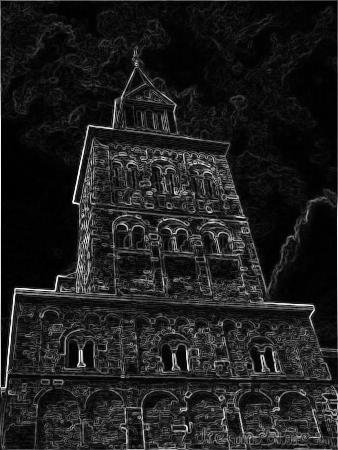
\includegraphics[width=1.4in]{churchout.jpg}
\hspace{.1in}
\end{figure}
\end {frame}

\begin{frame}{Sobel Kernel}
The kernel used to create this edge detection is in two parts:


$K_X = \begin{pmatrix}
	-1 & 0 & 1\\
	-2 & 0 & 2\\
	-1 & 0 & 1\\
\end{pmatrix}$
$K_Y = \begin{pmatrix}
	-1 & -2 & -1\\
	0 & 0 & 0\\
	1 & 2 & 1\\
\end{pmatrix}$

\vspace{.4in}
$E = \sqrt(E_Y^2+E_Y^2)$ Where $E_X$ and $E_Y$ are the result of the convolution.

\end{frame}

\begin{frame}{Blur + Edge Detection}
One can combine these operations to find the major edges in an image.

\begin{figure}[ht]
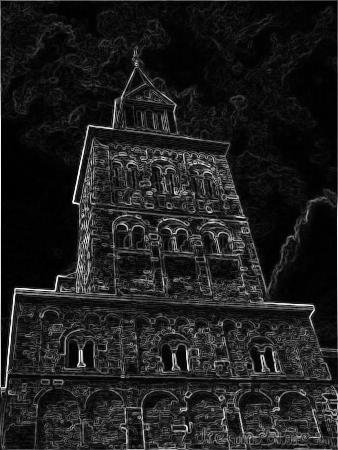
\includegraphics[width=1.3in]{churchout.jpg}
\hspace{.1in} 
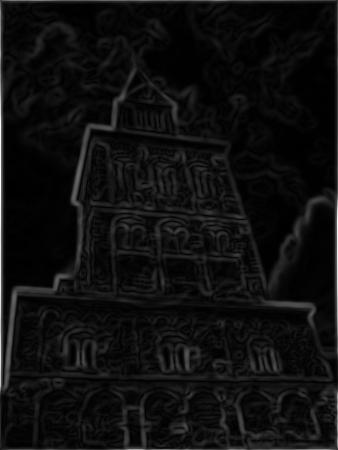
\includegraphics[width=1.3in]{churchoutbluredge.jpg}
\hspace{.1in}
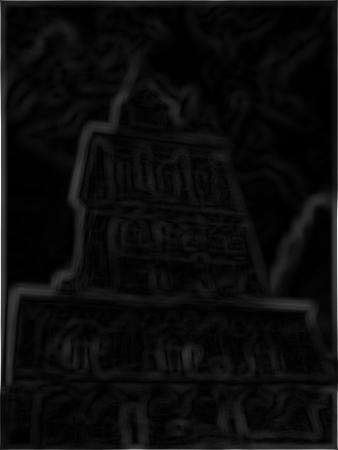
\includegraphics[width=1.3in]{churchoutblur2edge.jpg}
\hspace{.1in}
\caption{No Blur, Blur, $\sigma = 2$, $\sigma = 4$}
\end{figure}

\end{frame}

\begin{frame}{Color}
Our next feature that we implemented was color controls per channel. This would let us control how much of one color there is as well as increase or decreases brightness, changing all channels. This can be done by simply adding values to the matrix at each channel.

\begin{figure}[ht]
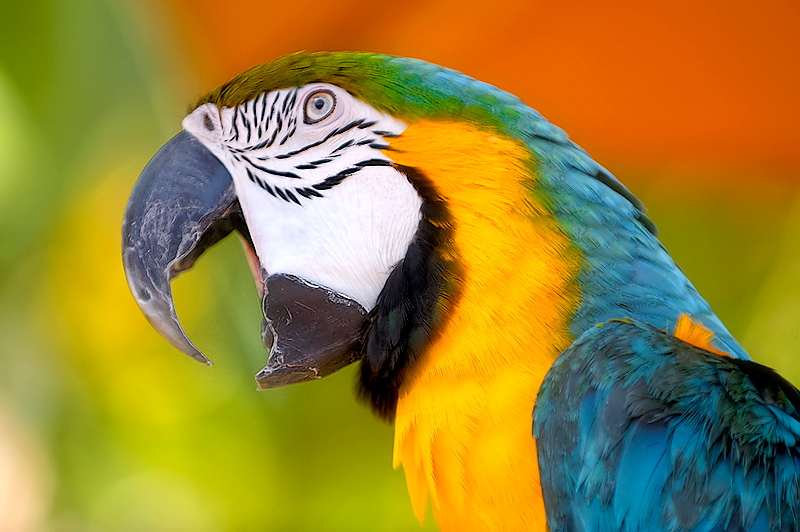
\includegraphics[width=1.4in]{parrot.jpg}
\hspace{.1in} 
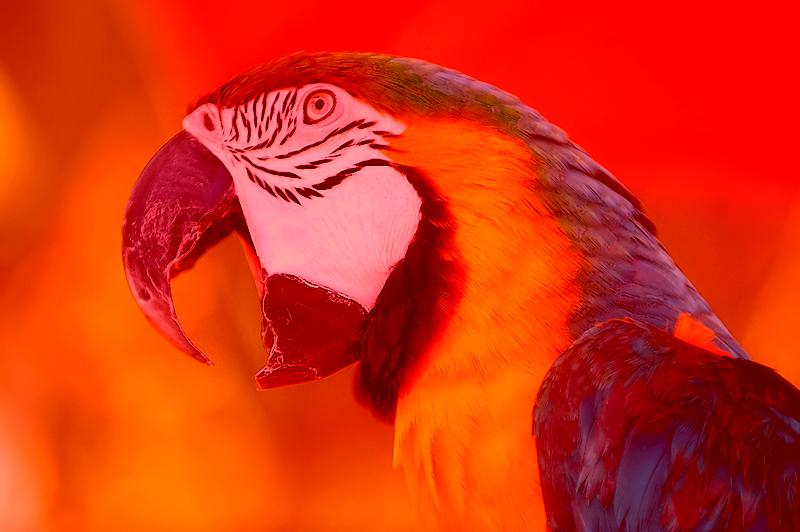
\includegraphics[width=1.4in]{parrotout1.jpg}
\hspace{.1in}
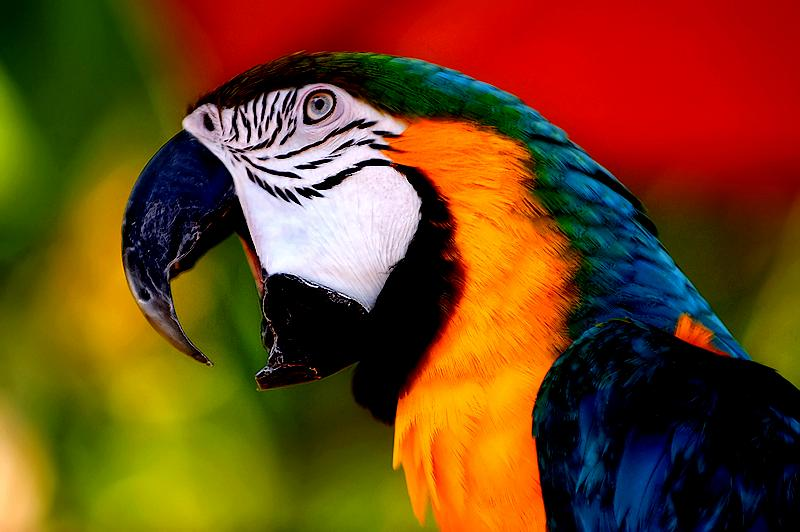
\includegraphics[width=1.4in]{parrotout2.jpg}
\hspace{.1in}
\caption{In order from left to right, original image, red increased with green and blue decreased, all channels decreased.}
\end{figure}

\end{frame}

\end{document}
